% !TeX spellcheck = en_US

\documentclass[]{report}

%%%%%%% USEPACKAGES %%%%%
\usepackage{amsmath,amssymb}
\usepackage{graphicx} 
\usepackage{tikz}
\usetikzlibrary{shapes,arrows,positioning,calc}
\usepackage{cleveref}
\usepackage{diffcoeff,physics}
\usepackage{todonotes}
\setuptodonotes{inline}

%%% THEOREMS %%%%
\newtheorem{defi}{Definition}

%%%%% COMMANDS %%%%%%%
\newcommand{\NN}[0]{\mathbb{N}}
\newcommand{\ZZ}[0]{\mathbb{Z}}
\newcommand{\RR}[0]{\mathbb{R}}
\newcommand{\CC}[0]{\mathbb{C}}

%opening
\title{Trying to learn Control Theory}

\begin{document}
\tikzset{
	block/.style = {draw, fill=white, rectangle, minimum height=3em, minimum width=3em},
	tmp/.style  = {coordinate}, 
	sum/.style= {draw, fill=white, circle, node distance=1cm},
	branch/.style= {draw, fill=black, circle, node distance=1cm},
	pinstyle/.style = {pin edge={to-,thin,black}}
}

\maketitle
\tableofcontents

\chapter{Definitions}
\begin{defi}[Controlled Variable and Manipulated Variable]
	The controlled variable is the quantity or condition that is measured and controlled. 
	The manipulated variable is the quantity or condition that is varied by the controller so as to affect the value of the controlled variable. 
	Normally, the controlled variable is the output of the system.
	Control means measuring the value of the controlled variable of the system and applying the manipulated variable to the system to correct or limit the measured value from a desired value.
\end{defi}
\begin{defi}[Plant]
	A plant may be a piece of equipment, perhaps just a set of machine parts functioning together, the purpose of which is to perform a particular operation. 
	We can call any physical object to be controlled (such as a mechanical device, a heating furnace, a chemical reactor, or a spacecraft) a plant.
\end{defi}
\begin{defi}[Disturbance]
	A disturbance is a signal that tends to adversely affect the value of the output of a system. 
	If a disturbance is generated within the system, it is called internal, while an external disturbance is generated outside the system and is an input.
\end{defi}
\begin{defi}[Feedback Control]
	Feedback control refers to an operation that, in the presence of disturbances, tends to reduce the difference between the output of a system and some reference input and does so on the basis of this difference. 
	Here only unpredictable disturbances are so specified, since predictable or known disturbances can always be compensated for within the system.
\end{defi}
\begin{defi}[Closed Loop]
	In a closed-loop control system the actuating error signal, which is the difference between the input signal and the feedback signal (which may be the system output itself or a function of it and its derivatives and/or integrals), is fed to the controller so as to reduce the error and bring the output of the system to a desired value.
	The term closed-loop control always implies the use of feedback control action in order to reduce system error, thus, in practice, the terms feedback control and closed-loop control are used interchangeably. 
\end{defi}
\begin{defi}[Open Loop]
	Those systems in which the output has no effect on the control action are called open-loop control systems. 
	In other words, in an open-loop control system the output is neither measured nor fed back for comparison with the input. 
	One practical example is a washing machine. 
	Soaking, washing, and rinsing in the washer operate on a time basis. 
	The machine does not measure the output signal, that is, the cleanliness of the clothes.
	In the presence of disturbances, an open-loop control system will not perform the desired task. 
	Open-loop control can be used, in practice, only if the relationship between the input and output is known and if there are neither internal nor external disturbances.
\end{defi}
\begin{defi}[Mathematical Models]
	A mathematical model of a dynamic system is defined as a set of equations that represents the dynamics of the system accurately or, at least, fairly well. 
	Note that a mathematical model is not unique to a given system. 
	A system may be represented in many different ways and, therefore, may have many mathematical models, depending on one's perspective.
	The dynamics of many systems, whether they are mechanical, electrical, thermal, economic, biological, and so on, may be described in terms of differential equations.
	Depending on the particular system and the particular circumstances, one mathematical model may be better suited than other models. 
	For example, in optimal control problems, it is advantageous to use state-space representations. 
	On the other hand, for the transient-response or frequency-response analysis of single-input-single-output, linear, time-invariant systems, the transfer function representation may be more convenient than any other. 
\end{defi}
\begin{defi}[Linear Systems]
	A system is called linear if the principle of superposition applies. 
	The principle of superposition states that the response produced by the simultaneous application of two different forcing functions is the sum of the two
	individual responses.
\end{defi}
\begin{defi}[State]
	The state of a dynamic system is the smallest set of variables (called state variables) such that the knowledge of these variables at $t=t_0$, together with the knowledge of the input for $t\ge t_0$, completely determines the behavior of the system $\forall ~~t\ge t_0$.
	Note that the aforementioned state variables need not be physically measurable or observable quantities, although it would be nice if they are.
\end{defi}
\begin{defi}[State Vector and State Space]
	If $n$ state variables are required to fully describe the behavior of a system, then they may be considered the components of an $n$ dimensional state vector $\mathbf{x}(t)$, which describes the state at any time $t$. 
	Consequently, the state space is the $n$-dimensional space whose coordinates consist of the state variables. 
	Any point in state space corresponds to a system state and a state vector. 
\end{defi}
\chapter{Mathematical Modeling of Dynamical Systems}
An example of a closed-loop system is shown in \cref{fig:closedloop}.
\begin{figure}
	\centering
	\begin{tikzpicture}[auto, node distance=2cm]
		\node [tmp, name=rinput] (rinput) {};
		\node [sum, right of=rinput] (sum) {$-$};
		\node [block, right of=sum] (system) {$G(s)$};
		\node [block, below of=system] (controller) {$H(s)$};
		\node [tmp, right of=system] (branch) {};
		\node [tmp, right of=branch] (output) {};
		\node [tmp, below of=controller] (tmp1){$H(s)$};
		\draw [->] (rinput) -- node{$r(s)$} (sum);
		\draw [->] (sum) --node[name=z,anchor=north]{$e(s)$} (system);
		\draw      (system) -- node{$y(s)$} (branch);
		\draw [->] (branch) -- node{$y(s)$} (output);
		\draw [->] (branch) |- node{$y(s)$} (controller);
		\draw [->] (controller) -| node[anchor=north]{$b(s)$} (sum);
	\end{tikzpicture}
	\caption{A closed-loop system.}\label{fig:closedloop}
\end{figure}
Note that, here, $G(s)$ may be interpreted as a plant, while $H(s)$ may represent a sensor measuring $b(s)$ from the plant output. 
Thus, we can define the \textit{open-loop transfer function} as
\begin{equation}
	\text{open-loop transfer function} = \frac{b(s)}{e(s)} = \frac{H(s)e(s)G(s)}{e(s)} = H(s)G(s),
\end{equation}
and the \textit{feedforward transfer function} as
\begin{equation}
	\text{feedforward transfer function} = \frac{y(s)}{e(s)} = \frac{e(s)G(s)}{e(s)} = G(s).
\end{equation}
Finally, we may also write the \textit{closed-loop transfer function}
\begin{equation}
	\text{closed-loop transfer function} = \frac{y(s)}{r(s)} = \frac{G(s)}{1+G(s)H(s)}
\end{equation}

\section{State Space}
After linearization around the operating point, write
\begin{align}
	\mathbf{\dot{x}}(t) &= \mathbf{A}(t)\mathbf{x}(t) + \mathbf{B}(t)\mathbf{u}(t),\label{eq:statesp}\\
	\mathbf{y}(t) &= \mathbf{C}(t)\mathbf{x}(t) + \mathbf{D}(t)\mathbf{u}(t),\label{eq:sysout}
\end{align}
where $\mathbf{A}(t)\in\CC^{n\cross n}$ is called the state matrix, $\mathbf{B}(t)\in\CC^{n\cross q}$ the input matrix, $\mathbf{C}(t)\in\CC^{k\cross n}$ the output matrix, and $\mathbf{D}(t)\in\CC^{k\cross q}$ the direct transmission matrix.
The state space, input and output vectors are denoted as $\mathbf{x}(t)\in\CC^{n}$, $\mathbf{u}(t)\in\CC^{q}$ and $\mathbf{y}(t)\in\CC^{k}$ respectively.
Note that the state, input, output and direct transmission matrices depend on the time $t$, as such \cref{eq:statesp,eq:sysout} describe a time varying system. 
\subsection{Controllability}
In practice, one may assume further modifications to the system to be intractable, i.e., the dynamics described by $\mathbf{A}$ as well as input modalities described by $\mathbf{B}$ have already been fixed.
This leaves solely the control input $\mathbf{u}(t)$ to manipulate the system.
Thus, using $\mathbf{A}$ and $\mathbf{B}$, it may be determined whether a system is controllable or not. 
Assuming an LTI system, we can write the control signal $\mathbf{u}(t)$ as a linear combination of the state vector components, i.e., 
\begin{equation}
	\mathbf{u}(t) = -\mathbf{K}\mathbf{x}(t),
\end{equation} 
which leads to 
\begin{equation}
	\mathbf{\dot{x}}(t) = (\mathbf{A} - \mathbf{BK})\mathbf{x}(t)
\end{equation}
\chapter{Automatic Controllers}
Previously, even though feedback was present, no specific or automated action was taken on the feedback signal.
This is where automatic controllers come in, which compare the actual value of the plant output with the reference input (desired value) and produce a control signal based on the deviation.
A general control system is shown in \cref{fig:controlsys}.
\begin{figure}
	\centering
	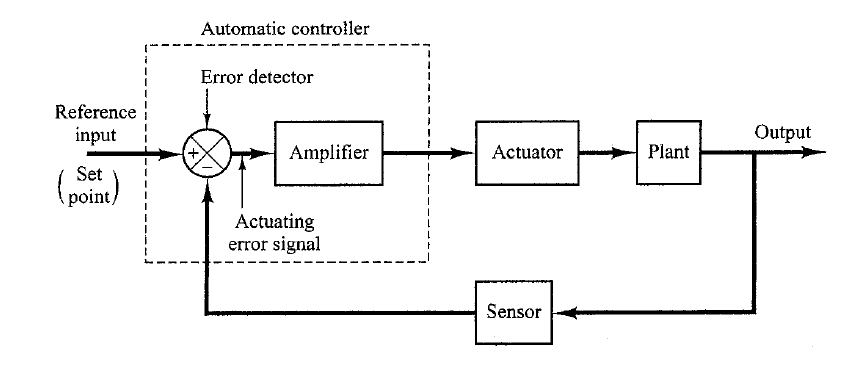
\includegraphics[width=0.7\linewidth]{graphics/controlSys}
	\caption{}
	\label{fig:controlsys}
\end{figure}
The manner in which the control signal $u(t)$ is produced is termed the \textit{control action}.
A large variety of control actions exist, such as binary (aka "on-off"), proportional, integral and derivative actions. 
What kind of controller to use must be decided based on the nature of the plant and the operating conditions, including considerations such as safety, cost, availability, reliability, accuracy, weight, and size.
\section{Proportional Integral Derivative Control}
In PID control, the resulting control signal \(u(t)\) from the error between the plant output and reference signal \(e(t)\) may be described as 
\begin{equation}
	u(t) = \underbrace{K_pe(t)}_{\text{Proportional}} + \underbrace{K_i\int_{0}^{t}e(\tau)\dd{\tau}}_{\text{Integral}} + \underbrace{K_d\diff{e(t)}{t}}_{\text{Derivative}},
\end{equation}
where $K_p$, $K_i$ and $K_d$ represent the gains for the proportional, integral and derivative control actions, respectively.
In the so-called \textit{standard form} $K_i$ and $K_d$ are replaced by $\frac{K_p}{T_i}$ and $K_pT_d$. 
This allows for a better physical interpretation since $T_i$ as well as $T_d$ have some physical meaning, with the former determining how long the controller tolerates a steady state error and the latter representing the time constant to approach the set point. 

The transfer function in the Laplace domain is given as 
\begin{equation}
	\mathcal{L}\left(\frac{u(t)}{e(t)}\right) = \frac{u(s)}{e(s)} = K(s) = K_p + K_i/s + K_ds.
\end{equation}

A block diagram of a PID system is given in \cref{fig:pid}.
\begin{figure}
	\centering
	\begin{tikzpicture}[auto, node distance=2cm]
		\node [tmp, name=rinput] (rinput) {};
		\node [sum, right of=rinput] (sum1) {};
		\node [block, right of=sum1] (controller) {$k_{p}$};
		\node [block, above of=controller,node distance=1.3cm] (up){$\frac{k_{i}}{s}$};
		\node [block, below of=controller,node distance=1.3cm] (rate) {$sk_{d}$};
		\node [sum, right of=controller,node distance=2cm] (sum2) {+};
		\node [block, right of=sum2,node distance=2cm] (system) 
		{Plant $G(s)$};
		\node [tmp, right of=system, node distance=2cm] (output) {};
		\node [tmp, below of=controller] (tmp1){$H(s)$};
		\draw [->] (rinput) -- node{$r(s)$} (sum1);
		\draw [->] (sum1) --node[name=z,anchor=north]{$e(s)$} (controller);
		\draw [->] (controller) -- (sum2);
		\draw [->] (sum2) -- node{$u(s)$} (system);
		\draw [->] (system) -- node [name=y] {$y(s)$}(output);
		\draw [->] (z) |- (rate);
		\draw [->] (rate) -| (sum2);
		\draw [->] (z) |- (up);
		\draw [->] (up) -| (sum2);
		\draw [->] (y) |- (tmp1)-| node[pos=0.99] {$-$} (sum1);
	\end{tikzpicture}
	\caption{A block diagram of a PID controller.}\label{fig:pid}
\end{figure}
Note that, for this system, the closed loop transfer function results in
\begin{equation}
	H(s) = \frac{K(s)G(s)}{1+K(s)G(s)},
\end{equation}
where the system becomes unstable for $K(s)G(s) = -1$.
\subsection{Tuning}
\todo{how ? }
\end{document}
